\documentclass[conference]{IEEEtran}
\IEEEoverridecommandlockouts
% The preceding line is only needed to identify funding in the first footnote. If that is unneeded, please comment it out.
\usepackage{cite}
\usepackage{amsmath,amssymb,amsfonts}
\usepackage{algorithmic}
\usepackage{graphicx}
\usepackage{textcomp}
\usepackage{siunitx}
\usepackage{xcolor}
\def\BibTeX{{\rm B\kern-.05em{\sc i\kern-.025em b}\kern-.08em
    T\kern-.1667em\lower.7ex\hbox{E}\kern-.125emX}}
\begin{document}

\title{Proposal on Mapping Robot*\\
{\footnotesize \textsuperscript{*}Note: This is a course project proposal for Robotics (CS283) in ShanghaiTech University in Fall 2019.}
}

\author{
% \IEEEauthorblockN{Xiting Zhao}
% \IEEEauthorblockA{\textit{School of Information Science and Technology} \\
% \textit{ShanghaiTech University}\\
% Shanghai, China \\
% zhaoxt@shanghaitech.edu.cn}
% \and
% \IEEEauthorblockN{Zhijie Yang}
% \IEEEauthorblockA{\textit{School of Information Science and Technology} \\
% \textit{ShanghaiTech University}\\
% Shanghai, China \\
% yangzhj@shanghaitech.edu.cn}
% \and
% \IEEEauthorblockN{Haochuan Wan}
% \IEEEauthorblockA{\textit{School of Information Science and Technology} \\
% \textit{ShanghaiTech University}\\
% Shanghai, China \\
% wanhch@shanghaitech.edu.cn}
Xiting Zhao\textsuperscript{1}, Zhijie Yang\textsuperscript{1} and Haochuan Wan\textsuperscript{1}
\thanks{\textsuperscript{1}All authors are with the School of Information Science and Technology, 
ShanghaiTech University, China.
        {\tt\small [zhaoxt, yangzhj, wanhch]@shanghaitech.edu.cn}}%
}

\maketitle

\begin{abstract}
This part of paper presents an approach to synchronizing different types of sensors which are installed on mapping robot.
\end{abstract}

\begin{IEEEkeywords}
Sensor Synchronization
\end{IEEEkeywords}

\section{Introduction}
For autonomous robots, the ability of getting from one place to another place is the most important capability. In order to realize this capability, Simultaneous Localization and Mapping (SLAM) system is often used and the result of SLAM is positively correlated with the quality of input data. To get better data, more sensors are used to collect information from environment. In our project, we installed an epic number of sensors, 10 RGB monocular cameras, 4 Lidars, 1 onmidirectional camera, 2 event cameras, 1 IMU and even IR cameras. However, as the number of sensors increases, the problem about synchronization between sensors is raised because synchronized system can lead sensors collect data at different time which results in errors in the generated map. In our project, we will migrate the existing synchronization on the existing mapping robot to the new one.

\section{State of the Art}

\subsection{Associated Datasets --- by Zhijie Yang}
ICL-NUIM dataset \cite{ICL-NUIM} mainly focused on RGB-D camera with handheld perspective within simulated indoor environments. The ground truth of this dataset comes from the model of the room. 

Robot@Home dataset \cite{Robot@Home} consists of the data stream comes from 4 RGB-D camera and 2 2D Lidar, but there is no pose ground truth. % But it is said to have pose ground truth via algorithm in the table?! 
CoRBS dataset\cite{CoRBS} is the first to have ground truth of camera trajectory and 3D model of the scenes. The camera is also upgraded to Microsoft Kinect v2 compared to TUM-RGBD dataset launched in 2012. The RGB resolution is $1920\times 1080@$30Hz and the depth cloud also revolves at 30Hz and have $512\times 424$ pixels in each frame. The tracking system generates 3D pose ground truth at 120Hz with error of 0.39mm.

Oxford RobotCar dataset\cite{RobotCar} is a dataset with four types of heterogeneous sensors mounted on a ground vehicle. The total mileage of this dataset covers more than 1000 kilometers. The scenes are within Oxford city, while most of them are repetition traverses along a route in Oxford. Its video stream consists of a stereo camera built up with three monocular RGB cameras, each equipped with a 2.67mm fisheye lens, obtaining \ang{180} field of view (FOV). The depth data are captured through two 2D Light Detection and Ranging sensors (Lidar) and a four-beam 3D Lidar. The two 2D Lidars are mounted to make the scans perpendicular to the ground, making it have a complete scan of the surroundings in a ``push-broom" manner. The 3D Lidar is mounted facing to the front, as a common configuration focusing the depth information in the front direction. The platform is also equipped with a 6 degree of freedom (DOF) IMU and GPS/GLONASS system reports its position at 50Hz. The three monocular cameras are synchronized at 11.1Hz frame rate, as the stereo camera produces 16Hz. The Lidar scans at 12.5Hz. All these sensors have their clock calibrated using TICSync. 

\subsubsection{ROS Package: velodyne --- by Zhijie Yang}
The ROS velodyne package is a set of packages consists of ``velodyne\_drive'', ``velodyne\_laserscan'', ``velodyne\_msgs'',  ``velodyne\_pointcloud'' and some utilities in directory ``velodyne''. The ``velodyne\_drive'' is the driver for the velodyne laser scanner. It is written in the ``node'' and ``nodelet'' manner. It deals with different models of velodyne Lidars and parse the TCP packets into scanning data. ``velodyne\_laserscan'' subscribes from topic ``velodyne\_points'' converts them into type of ``LaserScan'' and publishes them out. ``velodyne\_msgs'' defines the data structure of ``VelodynePacket'' and ``VelodyneScan'', where the former one has a time stamp and an 1206-element uint8 array as field for data, while the latter one has a ROS standard message header and an array of ``VelodynePacket'' with unpredefined length. The ``velodyne\_pointcloud'' packet is the one converts ``VelodynePackets'' into point clouds using pointcloud2 library. This combination of velodyne packages works as a whole --- the bottom layer driver acquires the TCP packets from via the ethernet, the laserscan package process the scans, the msgs package defines the messages types and the pointcloud package generats the ros-usable pointcloud2 point clouds. 

This packages is also simple to use --- clone it from github (https://github.com/ros-drivers/velodyne) into the src directory of a catkin work space, run catkin\_make, source the setup.bash, and it is done. 

\subsection{Synchronization --- by Wan Haochuan}
	In some previous works, most of approaches of synchronization just stayed on the level of software. Hang Hu \cite{1} mainly used ROS nodes to synchronize on software level. They realized the synchronization between cameras, LIDARs and GPS. However, the approach they provided focus on calibrating data rather synchronizing when sensors generating data.
	In \cite{Olson2010A}, a solution based on math calculation is introduced. It is a passive method to synchronize by eliminating transmission error between sensor data, which is a low-cost way to realize synchronization.
	A system \cite{Amundson2006Time} is designed for heterogeneous sensor networks is used to synchronize time. In this work, authors designed both software and hardware for synchronization. Software guarantees sensors receive signal at the same time and hardware like phase-locked loop is to correct time when errors occur.
	\par
	\begin{figure}
		\centering
		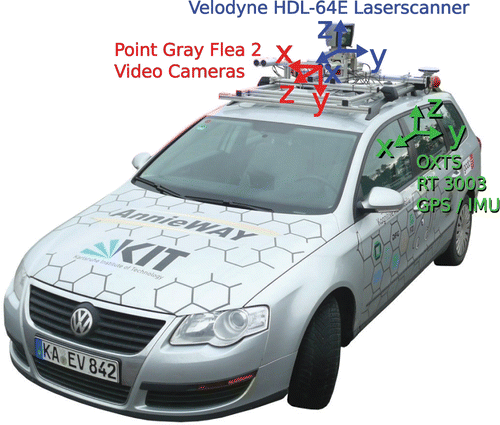
\includegraphics[width=.4\textwidth]{kitti_car.png}
		\caption{KITTI car}
		\label{car}
	\end{figure}

	By Georgios Litos's work \cite{Litos2006Synchronous}, a software-based system is provided. This method concerns cameras which are installed on different computers, and these computers are connected with NTP to get correct time. In order to trigger cameras at the same time, an estimate $L$ of how much time is required for cameras data is broadcast to all computers. Though time error will occur when the message propagate, yet each computer can calculate the time to wait and trigger the camera at the right time. In this case, the system can be used in a long distance sensor synchronization with NTP. But disadvantages are also existed if this system is applied on mapping robot directly. First, the distance between cameras on mapping robot is much closer so that to trigger different cameras with different computers is a waste. Second, this method can just synchronize trigger sensors, like camera and IMU. But there is another type of sensor by timestamp like pps and NMEA data which cannot be triggered, such as LIDAR and GPS. Third, the NTP can get a millisecond accuracy, which cannot meet the requirement of mapping robot in that some sensors like IMU should synchronized by a 200Hz signal. However, this work \cite{Litos2006Synchronous} provides a experiment which can evaluate the synchronization. They use a LED array controlled by a MircoChip. This array has 4 rows of 10 LEDs that can correspond to 1000ms, 100ms 10ms and 1ms granularities. Compared a 100Hz CRT screen which just provides 10ms accuracy, the LED array has an edge. By photographing the LED array, we can get the time of shot and judge the result of synchronization. This experiment method can evaluate some photosensitive sensor like cameras, but sensors such as IMU and LIDAR cannot be evaluated in this experiment.
	\par
	KITTI dataset \cite{Geiger2013IJRR} is one of the most famous opensource dataset regarding on autonomous driving. The main function of KITTI is collecting data from real world to build map for autonomous. Though the raw data is not in formal of ROS bag, yet we can convert it to rosbag easily by "kitti2bag" in python. And here we can use a ROS package which is "kitti\_to\_rosbag". By this ROS package, KITTI dataset raw data can be converted to a ROS bag and allows a library for direct access to poses, Velodyne scans and images. The car used by KITTI is equipped with a HDL-64E 3D Lidar, gray scale and RGB stereo cameras, which is show in Fig \ref{car}. All the Lidar and the cameras are synchronized and generates data at 10Hz. Global positioning system (GPS) and IMU data are also included in this dataset with 100Hz. The synchronization between GPS and IMU is not hardware-level synchronized with the camera or the Lidar. They use the time stamp to synchronize among them. There are six categories in KITTI and they are city, residential, road, campus, person and calibration.	KITTI dataset is also used to evaluate the performance of computer vision technology such as stereo, optical flow, visual odometry, 3D object detection and 3D tracking in the vehicle environment. KITTI contains real-world image data from scenes such as urban, rural, and highways, with up to 15 vehicles and 30 pedestrians per image, as well as varying degrees of occlusion and truncation. The entire data set consists of 389 pairs of stereo images and optical flow maps, 39.2km visual ranging sequences and images of 3D labeled objects, sampled and synchronized at 10Hz. For 3D object detection, the label is subdivided into car, van, truck, pedestrian, pedestrian (sitting), cyclist, tram and misc.

\begin{figure}
	\centering
	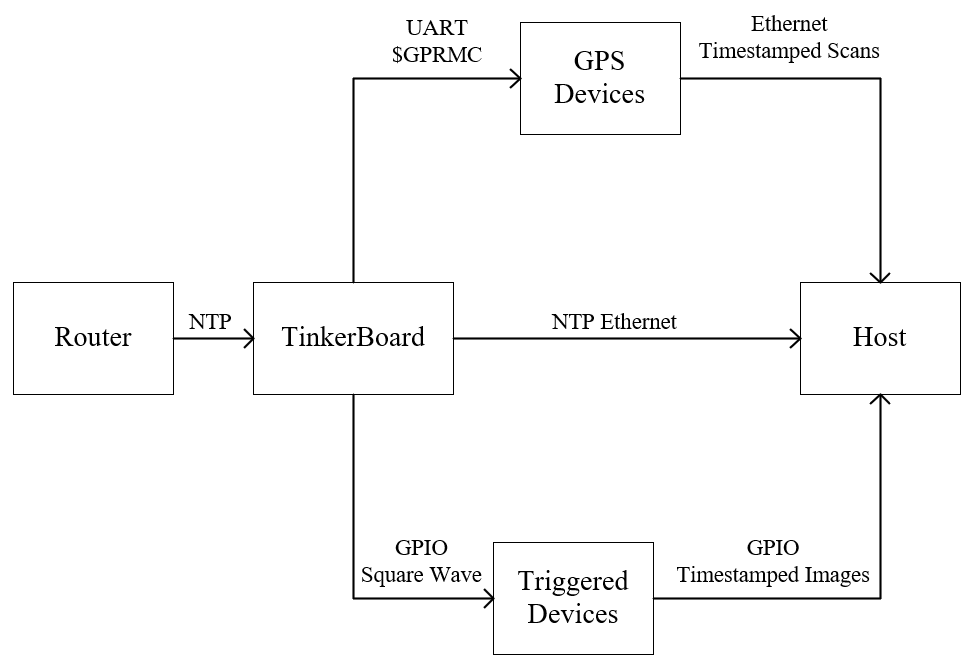
\includegraphics[width=.4\textwidth]{topology.png}
	\caption{Trigger \& Timestamp Spread Topology}
	\label{topology}
\end{figure}
\subsection{Software --- by Xiting Zhao}
There are some previous dataset, for example.
TUM-RGBD dataset \cite{TUM-RGBD}, as another indoor dataset, is captured by a synchronized Microsoft Kinect RGB-D camera both handheld and onboard of a ground robot. It has pose ground truth coming from a motion capture system at 100Hz. The images are with $640\times 480@30$Hz. 
EuRoC dataset\cite{EuRoC} is from a micro aerial vehicle (MAV). It is equipped with synchronized stereo monochrome cameras at 20 fps, inertia measurement unit (IMU) and has pose ground truth from laser tracking systems.
Zurich Urban MAV dataset \cite{Zurich_Urban_MAV} is also based on MAVs. Different from EuRoC, it is recorded in outdoor environments. The data are also time synchronized.

Zurich Urban MAV dataset use the MAV capture system to record the data in urban streets of Zurich, Switzerland. They fly the MAV at 5-15 meters above the ground. Their capture system is on a Fotokite quadrotor with a lot of sensors including barometer, gyrometer, accelerometer and GPS receiver synchronized with autopilot board and the cameras. It record the image at 1920 x 1080 and 30 fps. It use the GoPro Hero 4 to record the image. To get the ground truth pose of MAV, they performed an accurate photogrammetric 3D reconstruction using the Pix4D software. The GPS location is used for initial position in its ground truth pose calculation algorithm. The accuracy of the GPS pose is not so accurate because of the shadow of the building in the urban area. After that, they use the bundle adjustment algorithm with huge amount of 2D and 3D camera point to optimize the pose result and get a more accurate pose as the ground truth. So its ground truth comes from algorithms instead of directly from the capture system. In their dataset, they also have the ground Google Street View images which may be useful for the matching between the MAV image and the ground image. They also provide the calibration of the sensors including the Camera, the IMU, the GPS and the body of MAV. Their dataset are recorded in the raw data, but they provide a parsing algorithm to replay the data to the ROS platform.

We will use the ROS image\_transport package. The image\_transport package is used to subscribe to and publish images. When it subscribe or publish the image, it use the image\_transport\_plugin to compress and uncompress the image. In default, it provide three image\_transport\_plugin, which are the JPEG compression, the PNG compression and the Theora streaming video. The JPEG and PNG compression image\_transport\_plugin just use the OpenCV JPEG and PNG encoder and decoder to process the subscribed image. The OpenCV JPEG encoder and decoder use the libjpeg or the libjpeg-turbo library. The OpenCV PNG encoder and decoder use the libpng library. However all these image\_transport\_plugin are single thread and are very slow. According to the test, it can compress the 2448 x 2048 image at less than 50 fps at JPEG compression quality 90, when working on Intel i7 8700 at single thread. When it comes to the PNG image\_transport\_plugin, it can only compress the 2448 x 2048 image at less than 5 fps, when working on Intel i7 8700 at single thread. The most slow is the Theora image\_transport\_plugin, it can only compress the 2448 x 2048 image at less than 1 fps, when working on Intel i7 8700 at single thread. But for the date rate, the Theora as a video compressing format has the lowest data rate. The JPEG has a bit higher than that, as it is a compression with lost of the information. The PNG compression has the highest data rate.

\section{System Description}
\subsection{Synchronization}
	The core of the synchronization is TinkerBoard which broadcast triggering signals and NMEA message for two different kinds of sensors ------ Triggered devices and GPS devices. Triggered devices includes cameras at 10Hz, tracking system at 30Hz and IMU at 200Hz; GPS devices are LIDARs, Velodyne HDL-32E, which is synchronized by a PPS and message of \$GPRMC every second. The clock of TinkerBorad is synchronized by NTP with the host. To control different cameras with same signal, a PCB is designed to broadcast signal from one signal and convert 3.3V to 5V. The whole system is a hardware-level synchronization and showed in Fig \ref{topology}. 
\subsection{Software}
   We will implement the reflection detection and multi-thread JPEG compression on the robot. The reflection detection\cite{zhao2019mapping} use the dual return from Lidar and the intensity heap method to detect the reflection from the glass. It will improve the quality of the mapping. We also modify the image transport plugin to use multi threading to compress the JPEG image. So we can archive higher compress speed of the image.
\subsection{Super Accuracy}
    We will obtain ground truth pose information using a motion capture system with mean error less than 0.5mm. This ensures we have a pose to be considered as ground truth and we can just superpose point clouds over and over according to the transform calculated using such system. Motion compensation of the Lidar may also contribute to the accuracy since the robot is moving and the Lidar is a rotary sensor which always have some time difference within the one single scan. Using motion compensation may eliminate this error (distortion in point cloud) and thus providing a map with extremely high accuracy.
   
\section{System Evaluation}
\subsection{Synchronization}
	In order to evaluate the synchronization system, experiment are designed. Refer to the \cite{Litos2006Synchronous}, we will make a LED array controlled by MircoChip to represent time. Let cameras to photograph the LED array and compare pictures from different cameras to visualize delay between cameras.
	\par
	For other sensors, such as IMU and LIDAR, cannot detect their time error by the approach from \cite{Litos2006Synchronous} in that their own sensor properties. So, we should update the experiment system. Because IMU detects the movement of object and LIDAR uses light beams to scan objects around, so besides the LED array, we will build a rotating strick like a windmill with IMU installed. Put different LIDARs in front of the rotating strick to scan and achieve the  status of the system together with IMU. By comparing the different statuses from LIDARs and IMU at the same time, we can evaluate the synchronization system.
	\par
	However, there are some remaining problem of the experiment system. To compare system statuses from LIDARs and IMU, system calibration is essential. But for now it is difficult to calibrate LIDAR and IMU.
	
\subsection{Super Accuracy}
    This system using motion capture system as reference ground truth pose shall provide mapping results with great extent of accuracy improvement than the system using solely SLAM methods. The error of the map is measured by the root mean square (RMS) error compared to the ground truth map generated by FARO laser scanner.

\section{Work Plan}
	Nov 1: finish the synchronization system build.
	\par
	Nov 30: finish the experiment system build.
	\par
	Dec 30: test the whole system.

\begin{thebibliography}{00}
\bibitem{ICL-NUIM} A. Handa, T. Whelan, J. McDonald, and A. J. Davison. A Benchmark for RGB-D Visual Odometry, 3D Reconstruction and SLAM. In Proceedings of the IEEE International Conference on Robotics and Automation (ICRA), pages 1524–1531. IEEE, 2014
\bibitem{Robot@Home} Ruiz-Sarmiento, J. R., Cipriano Galindo, and J. González-Jiménez. "Robot@ home, a robotic dataset for semantic mapping of home environments." The International Journal of Robotics Research 36.2 (2017): 131-141.
\bibitem{TUM-RGBD} J. Sturm, N. Engelhard, F. Endres, W. Burgard, and D. Cremers. A Benchmark for the Evaluation of RGB-D SLAM Systems. In Proceedings of the IEEE/RSJ International Conference on Intelligent Robots and Systems (IROS), pages 573–580. IEEE, 2012
\bibitem{EuRoC} M. Burri, J. Nikolic, P. Gohl, T. Schneider, J. Rehder, S. Omari, M. W. Achtelik, and R. Siegwart. The EuRoC Micro Aerial Vehicle Datasets. The International Journal of Robotics Research (IJRR), 2016.
\bibitem{KITTI} A. Geiger, P. Lenz, C. Stiller, and R. Urtasun. Vision Meets Robotics: The KITTI Dataset. The International Journal of Robotics Research (IJRR), 32(11):1231–1237, 2013
\bibitem{Zurich_Urban_MAV} Andras Majdik and Charles Till and Davide Scaramuzza. The Zurich urban micro aerial vehicle dataset. The International Journal of Robotics Research (IJRR) 36 (2017): 269-273
\bibitem{TMU-VI} Schubert, David, et al. "The TUM VI Benchmark for Evaluating Visual-Inertial Odometry." arXiv preprint arXiv:1804.06120 (2018).
\bibitem{ADVIO} Cortés, S., Solin, A., Rahtu, E., \& Kannala, J. (2018). ADVIO: An authentic dataset for visual-inertial odometry. In Proceedings of the European Conference on Computer Vision (ECCV) (pp. 419-434).
\bibitem{CoRBS} O. Wasenmuller, M. Meyer, and D. Stricker. CoRBS: Comprehensive RGB-D benchmark for SLAM using Kinect v2. In IEEE Winter Conference on Applications of Computer Vision (WACV), pages 1–7. IEEE, 2016
\bibitem{RobotCar} Maddern, Will, et al. "1 year, 1000 km: The Oxford RobotCar dataset." The International Journal of Robotics Research (2016): 0278364916679498. 
\bibitem{Amundson2006Time}
Isaac Amundson, Manish Kushwaha, Branislav Kusy, Peter Volgyesi, Gyula Simon,
  Xenofon Koutsoukos, and Akos Ledeczi.
\newblock Time synchronization for multi-modal target tracking in heterogeneous
  sensor networks.
\newblock {\em Social Science Electronic Publishing}, 11(2):152--4, 2006.

\bibitem{Geiger2013IJRR}
Andreas Geiger, Philip Lenz, Christoph Stiller, and Raquel Urtasun.
\newblock Vision meets robotics: The kitti dataset.
\newblock {\em International Journal of Robotics Research (IJRR)}, 2013.

\bibitem{1}
h.~{Hu}, J.~{Wu}, and Z.~{Xiong}.
\newblock A soft time synchronization framework for multi-sensors in autonomous
  localization and navigation.
\newblock In {\em 2018 IEEE/ASME International Conference on Advanced
  Intelligent Mechatronics (AIM)}, pages 694--699, July 2018.

\bibitem{Litos2006Synchronous}
Georgios Litos, Xenophon Zabulis, and Georgios Triantafyllidis.
\newblock Synchronous image acquisition based on network synchronization.
\newblock In {\em Conference on Computer Vision \& Pattern Recognition
  Workshop}, 2006.

\bibitem{Olson2010A}
E.~Olson.
\newblock A passive solution to the sensor synchronization problem.
\newblock 2010.

\bibitem{zhao2019mapping}
Xiting Zhao and Zhijie Yang and Sören Schwertfeger
\newblock Mapping with Reflection -- Detection and Utilization of Reflection in 3D Lidar \newblock In {\em arXiv 1909.12483} 2019

\end{thebibliography}
\end{document}

